\documentclass{article}

\usepackage[spanish]{babel}
\usepackage{mathdots}
\usepackage{listings}
\usepackage{color}
\usepackage[numbers,sort&compress]{natbib}
\usepackage{graphicx}
\usepackage{subfigure}
\usepackage{url}
\usepackage{amsmath}
\usepackage{hyperref}
\usepackage[top=15mm, bottom=40mm, left=15mm, right=15mm]{geometry}
\setlength{\parskip}{2mm}
\setlength{\parindent}{0pt}

\setlength{\parskip}{2mm}
\setlength{\parindent}{0pt}
\definecolor{blue}{rgb}{0,0.6,0}
\definecolor{gray}{rgb}{0.3,0.3,0.3}
\definecolor{orange}{rgb}{0.8,0.4,0}
\definecolor{mostaza}{rgb}{0.9,0.8,0.1}

\lstset{ %
  language=R,                     % the language of the code
  basicstyle=\footnotesize,       % the size of the fonts that are used for the code
  numbers=left,                   % where to put the line-numbers
  numberstyle=\tiny\color{gray},  % the style that is used for the line-numbers
  stepnumber=1,                   % the step between two line-numbers. If it's 1, each line
                                  % will be numbered
  numbersep=5pt,                  % how far the line-numbers are from the code
  backgroundcolor=\color{white},  % choose the background color. You must add \usepackage{color}
  showspaces=false,               % show spaces adding particular underscores
  showstringspaces=false,         % underline spaces within strings
  showtabs=false,                 % show tabs within strings adding particular underscores
  frame=single,                   % adds a frame around the code
  rulecolor=\color{black},        % if not set, the frame-color may be changed on line-breaks within not-black text (e.g. commens (green here))
  tabsize=2,                      % sets default tabsize to 2 spaces
  captionpos=b,                   % sets the caption-position to bottom
  breaklines=true,                % sets automatic line breaking
  breakatwhitespace=false,        % sets if automatic breaks should only happen at whitespace
  title=\lstname,                 % show the filename of files included with \lstinputlisting;
                                  % also try caption instead of title
  keywordstyle=\color{orange},      % keyword style
  commentstyle=\color{blue},   % comment style
  stringstyle=\color{mostaza},      % string literal style
  escapeinside={\%*}{*)},         % if you want to add a comment within your code
  morekeywords={*,...}            % if you want to add more keywords to the set
} 

\author{1445183}
\title{Práctica 9: interacciones entre partículas}
\date{\today}

\begin{document}

\maketitle

\section{Objetivo}
Agregar masa a cada partícula generada en el código proporcionado por la \textit{práctica 9} lo cual genera atracciones además de las fuerzas causadas por las cargas y estudiar la distribución de las velocidades de las partículas, verificando gráficamente la relación entre la velocidad, la carga y la masa de las partículas.

\section{Descripción}
La masa se agrega siguiendo el ejemplo del código dado para agregar carga a las partículas \cite{elisaweb9} y se añade al \texttt{data.frame}, en la figura \ref{parmas} se puede observar las partículas generadas con masa y carga:
\begin{lstlisting}[language=R]
p <- data.frame(x = rnorm(n), y=rnorm(n), c=rnorm(n), m=rnorm(n))
mmax <- max(p$m)
mmin <- min(p$m)
p$m <- ((p$m - mmin)*(p$m - mmin) / (mmax - mmin))+1 #masa entre 1 y 5
\end{lstlisting}

\begin{figure}[h!]
\centering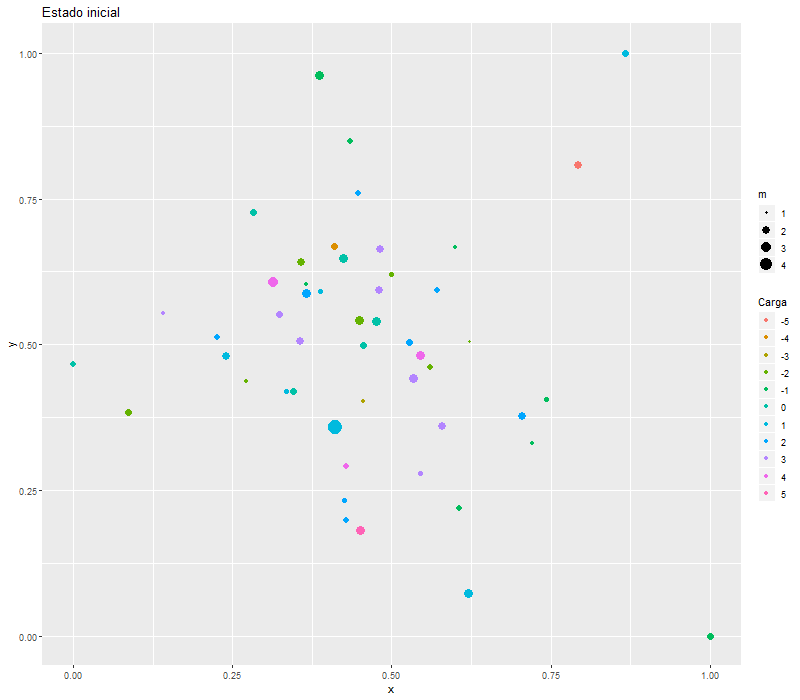
\includegraphics[width=120mm]{p9_t0.png}
\caption{Partículas con carga y masa}
\label{parmas}
\end{figure}

\newpage
Después la masa se añade a la función de \texttt{fuerza} para que interactúe junto con la carga al movimiento de las partículas:
\begin{lstlisting}[language=R]
fuerza <- function(i) {
  xi <- p[i,]$x
  yi <- p[i,]$y
  ci <- p[i,]$c
  mi <- p[i,]$m #masa
  fx <- 0
  fy <- 0
  for (j in 1:n) {
    cj <- p[j,]$c
    dir <- (-1)^(1 + 1 * (ci * cj < 0))
    dx <- xi - p[j,]$x
    dy <- yi - p[j,]$y
    factor <- dir * abs(ci - cj) / (sqrt(dx^2 + dy^2) + eps)
    fx <- fx - dx * factor
    fy <- fy - dy * factor
  }
  return(c(fx, fy)/(mi+1))
\end{lstlisting}

La velocidad se añade al \texttt{data.frame} con un vector que se relaciona con la masa, tomando en cuenta los valores obtenidos para \textit{x} y \textit{y} obtenidos en el \texttt{for} de las iteraciones.
\begin{lstlisting}[language=R]
p$v <- foreach(i = 1:n, .combine=c) %dopar% (xdifmax[i] + ydifmax[i])
p$v <- p$m * p$v
\end{lstlisting}
\newpage


\section{Resultados}
Para visualizar los resultados se consideran los pasos \textit{1, 25, 50, 75} y \textit{100}. En la figura \ref{fig2} se observa el movimiento de las partículas bajo la influencia de la carga y la masa.

\begin{figure}[h!]
\centering
\subfigure[]{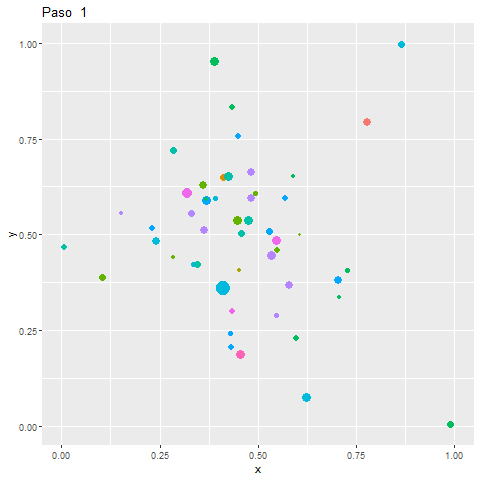
\includegraphics[width=60mm]{./p9_t001.png}}
\subfigure[ ]{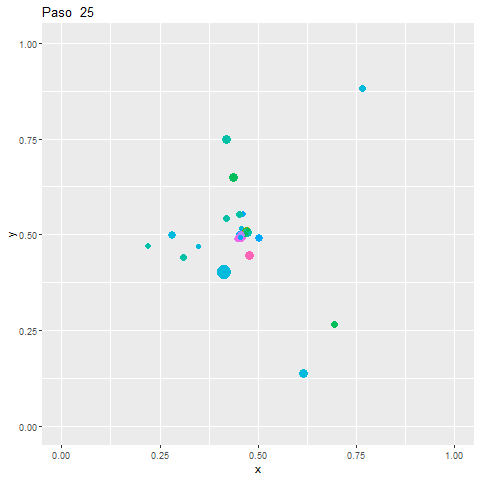
\includegraphics[width=60mm]{./p9_t025.png}}
\subfigure[]{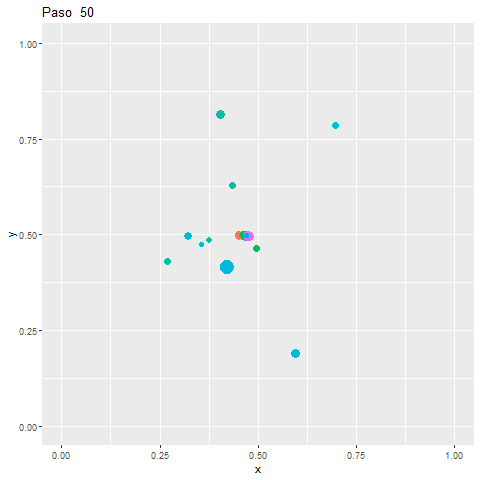
\includegraphics[width=60mm]{./p9_t050.png}}
\subfigure[]{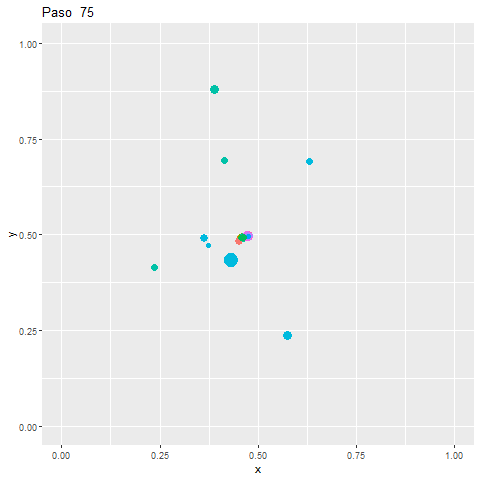
\includegraphics[width=60mm]{./p9_t075.png}}
\subfigure[]{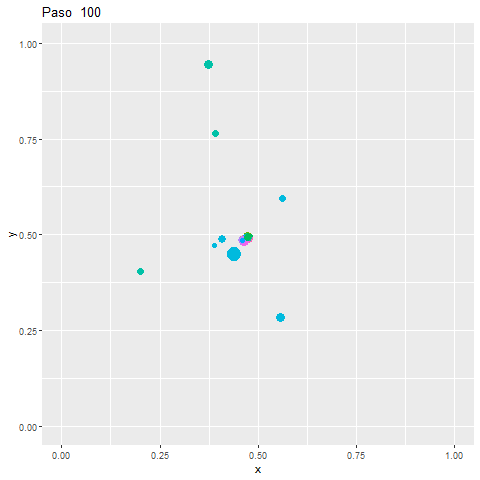
\includegraphics[width=60mm]{./p9_t100.png}}
\caption{Interacción de partículas}\label{fig2}
\end{figure}

En cuanto a la relación de la velocidad, carga y masa se puede observar en la figura \ref{fig3} que conforme aumentan los pasos, la distribución de velocidad-carga tiende hacia un mismo punto, en cambio en relación con la masa, no se ve una distribución uniforme \cite{plot9}.

\begin{figure}[h!]
\centering
\subfigure[]{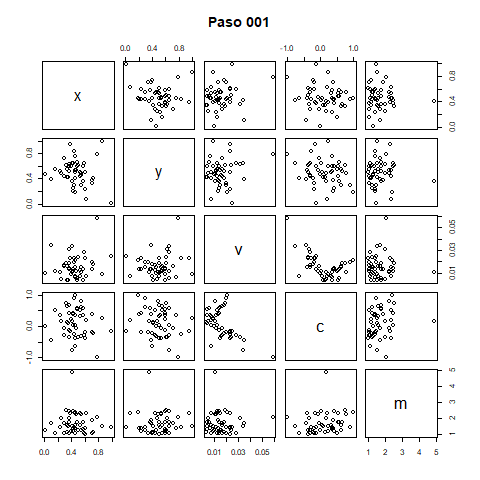
\includegraphics[width=80mm]{./p9_pairs001.png}}
\subfigure[ ]{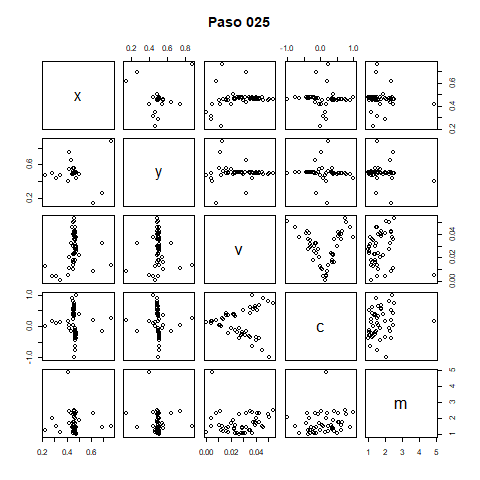
\includegraphics[width=80mm]{./p9_pairs025.png}}
\subfigure[]{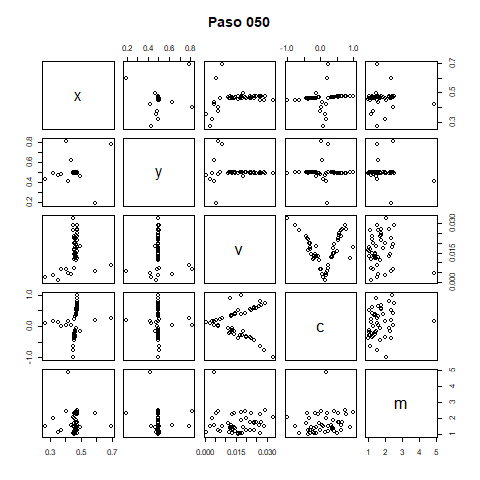
\includegraphics[width=80mm]{./p9_pairs050.png}}
\subfigure[]{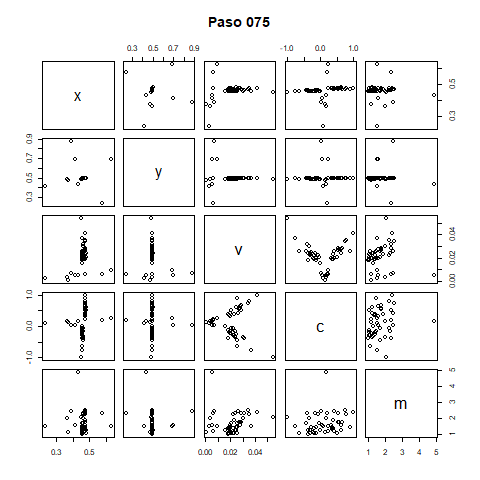
\includegraphics[width=80mm]{./p9_pairs075.png}}
\subfigure[]{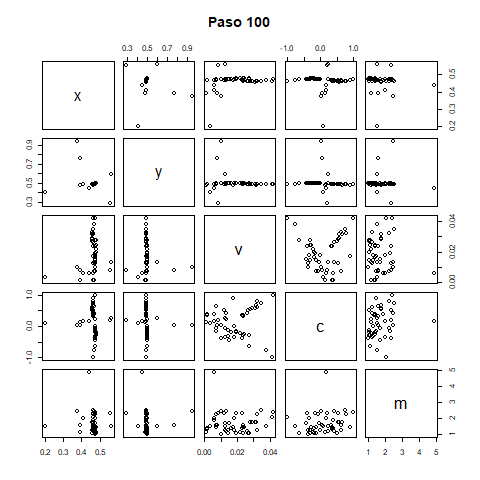
\includegraphics[width=80mm]{./p9_pairs100.png}}
\caption{Relación de velocidad, carga y masa de las partículas}\label{fig3}
\end{figure}

En las siguientes figuras se observa las distribuciones de velocidad en relación con la masa (figura \ref{fig4}) y en relación con la carga (figura \ref{fig5}).
\begin{figure}[!h]
\centering
\subfigure[]{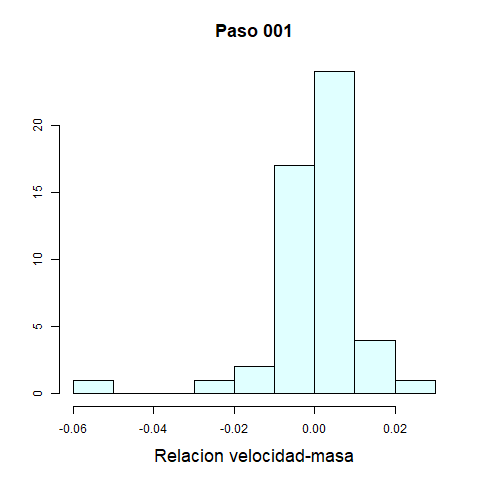
\includegraphics[width=60mm]{./p9_thism001.png}}
\subfigure[ ]{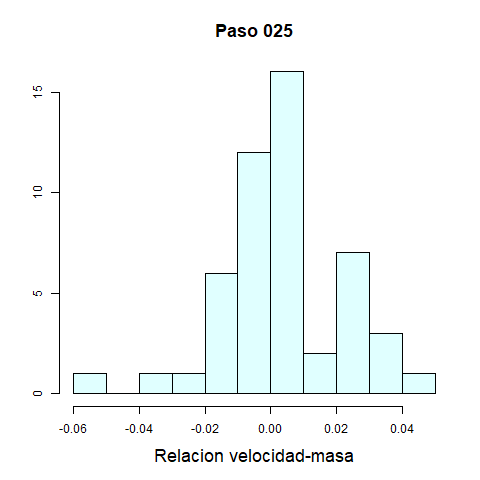
\includegraphics[width=60mm]{./p9_thism025.png}}
\subfigure[]{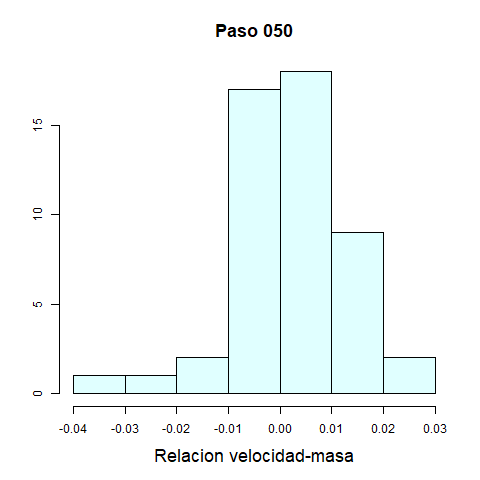
\includegraphics[width=60mm]{./p9_thism050.png}}
\subfigure[]{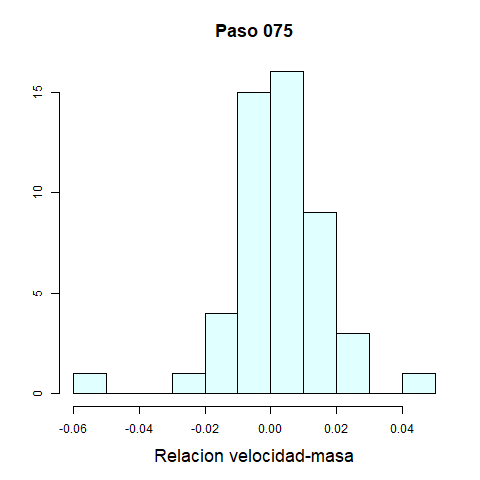
\includegraphics[width=60mm]{./p9_thism075.png}}
\subfigure[]{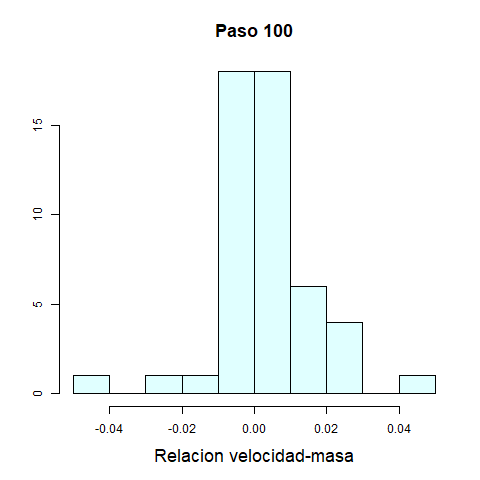
\includegraphics[width=60mm]{./p9_thism100.png}}
\caption{Distribución velocidad-masa}\label{fig4}
\end{figure}

\begin{figure}[h!]
\centering
\subfigure[]{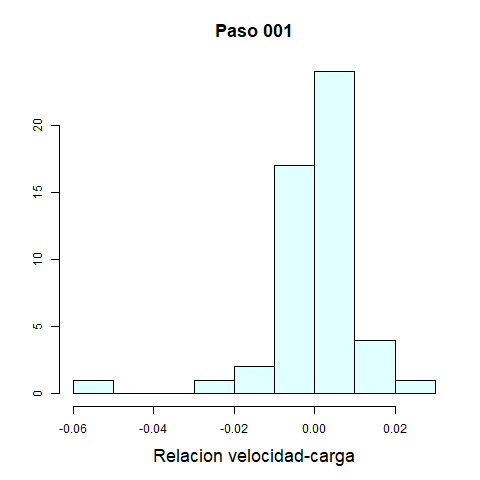
\includegraphics[width=60mm]{./p9_thisc001.png}}
\subfigure[ ]{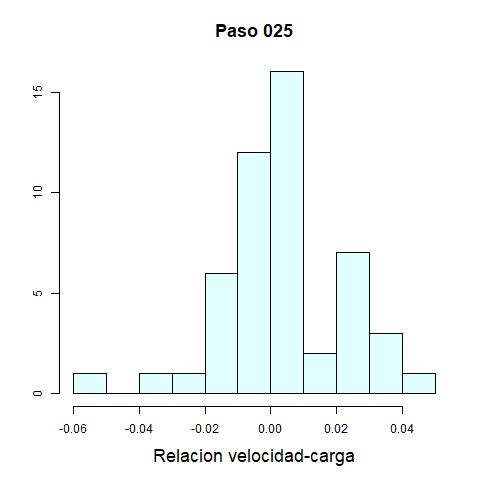
\includegraphics[width=60mm]{./p9_thisc025.png}}
\subfigure[]{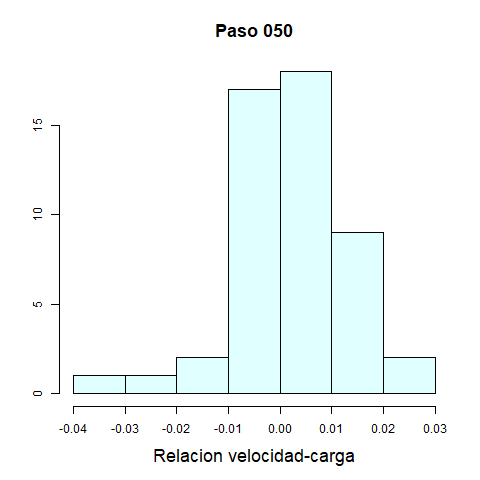
\includegraphics[width=60mm]{./p9_thisc050.png}}
\subfigure[]{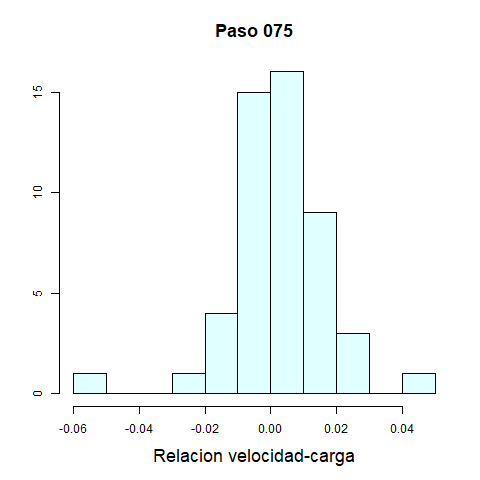
\includegraphics[width=60mm]{./p9_thisc075.png}}
\subfigure[]{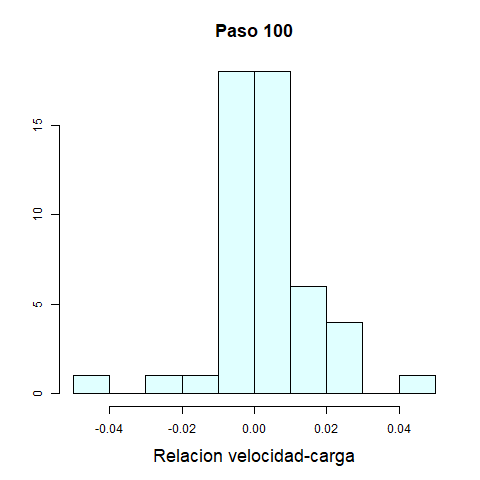
\includegraphics[width=60mm]{./p9_thisc100.png}}
\caption{Distribución velocidad-carga}\label{fig5}
\end{figure}



\newpage
\section{Conclusión}
La velocidad en relación con la carga tiene el mismo comportamiento para un valor absoluto de carga, la velocidad es menor cuando las cargas están cerca de cero, es decir, la fuerzas entre partículas es menor. La velocidad en relación con la masa tiene más influencia con masas pequeñas que con las grandes.
En el \textit{paso 100} algunas partículas ya no interactúan con las demás partículas y se alejan por las cargas concentradas en un punto, lo que afecta a la relación velocidad-carga y velocidad-masa.

\newpage
\bibliographystyle{plainnat}
\bibliography{bibliosimu}

\end{document}